\documentclass[a4paper,10pt, twocolumn, pre]{revtex4}
\usepackage[utf8]{inputenc}

\usepackage{amsmath}
\usepackage{caption}
\usepackage[toc,page]{appendix}
\usepackage{graphicx}
\bibliographystyle{naturemag}

\newcommand{\rvec}{\mathbf{r}}
\newcommand{\Rvec}{\mathbf{R}}
\newcommand{\xvec}{\mathbf{x}}
\newcommand{\dd}{\mathrm{d}}
\newcommand{\Pvec}{\mathbf{P}}
\newcommand{\mb}{\mathbf}
\newcommand{\overlap}[2]{\langle {#1}|{#2} \rangle}
\newcommand{\sandwich}[3]{\langle {#1}|{#2}|{#3}\rangle}

%opening

\begin{document}
\title{Project in FYS4411 - Hartree-Fock calculations on atoms and small molecules}
\author{Henrik Andersen Sveinsson}
\affiliation{Department of Physics, University of Oslo}
\date{\today}

\begin{abstract}
We apply the restricted Hartree-Fock method (RHF) to several atomic and molecular systems. We bechmark a Hartree-Fock solver using known correlation energies, and investigate how different GTO bases, STO-3G, STO-6G, 3-21G and 4-31G influence ground state energies and nuclei configurations.
\end{abstract}
\maketitle
\tableofcontents


\part{Introduction}
Hartree-Fock theory is an approach to the many-electron problem. It is widely used for finding an approximate wave function of a quantum mechanical system. Hartree-Fock calculations yield surprisingly good results with respect to ground state energies, when one takes into account that the coloumb-interaction between the electrons are done in a mean-field way. In this project, we study how different atomic and molecular systems behave within the Hartree-Fock approximation. We will look at He and Be atoms to make a first implementation of a HF-solver with atomic orbitals, and then move on to Gaussian Type Orbitals (GTO's). With GTO's, we will study more complicate systems, such as the water molecule. Our main aim is to bechmark s HF-solver against known ground state energies for various systems, but we will also look at equlibrium configurations and the actual electron distribution for selected systems. 
%%%%%%%%%%%%%%%%%%%%%%%
\part{Theory \& Methods}
%%%%%%%%%%%%%%%%%%%%%%%
\section{The Hartree-Fock method}
Here is a brief overview of the Hartree-Fock method. I will go into details on how to actually find optimal functions to minimize the \emph{Hartree-Fock functional}. 
\subsection{Approximations}
There are five main approximations in the Hartree-Fock method:
\begin{itemize}
 \item The Born-Oppenheimer approximation
 \item The solution is a linear combination of basis functions
 \item Each energy eigenfunction is assumed to be describable by a single Slater determinant
 \item A mean field approximation is implied. 
\end{itemize}

The two last approximations are the ones that differentiate the HF method from other similar methods. The HF-method leads us to the Hartree-Fock functional which reads:
\begin{equation}
	E[\Phi] = \sum_{\mu = 1}^N \langle \mu |h|\mu \rangle + \frac{1}{2} \sum_{\mu = 1}^N\sum_{\nu=1}^N \left[ \langle \mu\nu |\frac{1}{r_{ij}}| \mu\nu\rangle - \langle \mu\nu |\frac{1}{r_{ij}}| \nu\mu\rangle \right]
\end{equation}
Where the fuctions with greek letters are functions that if put into a slater determinant, will be our approximation to the electronic wave function. The goal is to find these functions. 

We begin by using the fact that electrons come in pairs, and that two electrons of opposite spin can occupy the same orbital state. This means we can only investigate \emph{closed shell} systems, and that the method we use is \emph{Restricted Hartree-Fock}. Our strategy will be to minimize the Hartree-Fock functional, i.e. find the optimal coefficients with respect to set of basis functions. The variational principle guarantees us that this will be an upper enstimate of the ground state energy of the system.



\section{Minimizing the Hartree-Fock functional}
We will apply some sort of variational scheme to the Hartree-Fock functional in order to find an optimal basis $\{\psi'\}$ for the single-particle wave functions. We use a unitary transformation to write the HF-equation for a different basis. This is explained in the appendix. We represent this new basis with latin letters, whereas the old basis is represented by greek letters. 
\begin{equation}
	E[\Psi] = \sum_{a=1}^N \langle a|h|a \rangle + \frac{1}{2} \sum_{ab}\left[  \langle ab |\frac{1}{r_{ij}}|ab \rangle - \langle ab | \frac{1}{r_{ij} }| ba\rangle \right]
\end{equation}

We now expand all these basis functions in the old basis:

\begin{align}
	E[\Psi] &= \sum_{a=1}^N \sum_\alpha \sum_\beta C_{a\alpha}^* C_{a\beta}\langle \alpha |h|\beta\rangle
	\nonumber \\
	&+
	\frac{1}{2} \sum_a \sum_b \sum_\alpha \sum_\beta \sum_\gamma \sum_\delta 
	C^*_{a\alpha} C^*_{b\beta} C_{a\gamma} C_{b\delta} \nonumber \\
	&\left[  \langle \alpha\beta |\frac{1}{r_{ij}}|\gamma\delta \rangle - \langle \alpha\beta | \frac{1}{r_{ij} }| \delta\gamma \rangle \right]
\end{align}

This takes us to:
\begin{equation}
	\sum_\gamma^N h_{\alpha\gamma}^{HF} C_{k\gamma} = \epsilon_k C_{k\alpha}
	\label{eq:hfsum}
\end{equation}

where 
\begin{equation}
	h_{\alpha\gamma}^{HF} = \langle \alpha |h|\gamma\rangle + \frac{1}{2}\sum_{a \beta \delta}  C^*_{a\beta}C_{a\delta} \left[ 
	\langle\alpha \beta|\frac{1}{r_{ij}}| \gamma \delta \rangle
	-
	\langle\alpha \beta|\frac{1}{r_{ij}}| \delta \gamma \rangle
	\right]
\end{equation}

We now take into account that two electrons can be in the same orbital state. According to \cite{thijssen2007computational} page 63, this changes $h^{HF}$ to:
\begin{equation}
	h_{\alpha\gamma}^{HF} = \sandwich{\alpha}{h}{\gamma} + \frac{1}{2}\sum_{a\beta\delta} C_{a\beta}C^*_{a\delta} (2\sandwich{\alpha\beta}{\frac{1}{r_{ij}}}{\gamma\delta}-\sandwich{\alpha\beta}{\frac{1}{r_{ij}}}{\delta\gamma} )
\end{equation}
In addition, the sum of equation \ref{eq:hfsum} now goes to $\frac{N}{2}$, which means we count two-electron states. To allow for non-orthogonal basis sets, we introduce the overlap matrix $\mb{S}$, such that the equation we need to solve is:
\begin{equation}
		\sum_\gamma^{N/2} h_{\alpha\gamma}^{HF} C_{k\gamma} = \epsilon_k S_{k\alpha}C_{k\alpha}
	\label{eq:hfsumfinal}
\end{equation}
This is effectively the \emph{Roothan equation}.

$h^{HF}$ gives rise to the \emph{Fock matrix}. Almost all the work in the HF-method is to find the Fock matrix. From there on, we have a self consistent set of equations, which can be solved iteratively with standard linear algebra software. I use Armadillo \cite{Sanderson2011} for this project. 


\section{Integral evaluations}
Now that we know how to set up the linear algebra problem of Hartree-Fock, we move on to the integral evaluations, since the brakets are integrals. At the end of the section, it is explained how the integrals go in to the method described above. 
This section about integral evaluations will follow Helgakers slides \cite{helgaker2006}. The necessary results for the implementation in this project are included. 
\subsection{Cartesian GTO's}
Cartesian Gaussians are on the form:
\begin{equation}
	G_a = G_{ikm}(a, \rvec_A) = x^i_A y^k_A z^m_A e^{-ar^2_A}
	\label{eq:gaussianprimitive}
\end{equation}
Where $r_A = |\rvec_A|$ is the distance to the origin of the Gaussian.


\subsection{Overlap integrals}
The overlap integrals $S_{ab} = \overlap{G_a}{G_b}$ are:
\begin{equation}
	S_{ab} = E_0^{ij}E_0^{kl}E_0^{mn}\left(\frac{\pi}{p}\right)^{\frac{3}{2}}
\end{equation}
Where $E_t^{ij}$ are Hermite coefficients. 
The Hermite coefficients can be found using recurrence relations. 
\begin{equation}
	E_0^{00} = e^{-\frac{q}{p}X_{AB}^2}
\end{equation}
We also know that $E_{t<0} = 0$ and $E_{t>i+j} = 0$
Where $p = a+b$ and $q = \frac{ab}{a+b}$.
Now, the recurrence relations are:
\begin{equation}
	E_t^{i+1,j} = \frac{1}{2p}E_{t-1}^{ij} + X_{PA}E_t^{ij} + (t+1) E_{t+1}^{ij}
\end{equation}
\begin{equation}
	E_t^{i, j+1} = \frac{1}{2p}E_{t-1}^{ij}+X_{PB}E_t^{ij} + (t+1)E_{t+1}^{ij}
\end{equation}

\subsection{Kinetic integrals}

Kinetic integrals are products of overlap integrals with some exponents changed.

\subsection{One-electron nuclear attraction integrals (Coulomb)}
The general form of these integrals are:
\begin{equation}
	V_{ab} = \sandwich{G_a(\rvec_A)}{\frac{1}{r_C}}{G_b(\rvec_B)}
\end{equation}

We know that this integral can be written:
\begin{equation}
	V_{ab} = \int \frac{\Omega_{ab}}{r}\dd \rvec  
\end{equation}
Rewriting in terms of hermite gaussians, we are able to separate this integral into a sum of products of hermite coefficients and one-center hermite integrals:
\begin{equation}
	V_{ab} = \sum_{t=0}^{i+j}E_{t}^{ij}\sum_{u=0}^{k+l}E_{u}^{kl}\sum_{v=0}^{m+n}E_{v}^{mn} \int \frac{\Lambda_{tuv}(\rvec_P)}{r_C} \dd \rvec
\end{equation}

The Hermite integral can be solved in terms of a boys functions $F_n(x)$ and recurrence relations, so that:
\begin{equation}
	V_{ab} = \frac{2\pi}{p}\sum_{tuv} E_{tuv}^{ab} R_{tuv}(p, \mb{R}_{PC})
\end{equation}
To find the $R$'s, we need \emph{Auxillary Hermite integrals} $R_{tuv}^n$, because they provide sufficient recursion relations to find the $R_{tuv}^0$'s that we are interested in.

Relevant recurrence relations for these integrals are:
\begin{align}
R_{t+1, u, v}^n = tR_{t-1, u, v}^{n+1} + A_xR_{tuv}^{n+1} \\
R_{t, u+1, v}^n = uR_{t, u-1, v}^{n+1} + A_yR_{tuv}^{n+1} \\
R_{t, u, v+1}^n = vR_{t, u, v-1}^{n+1} + A_zR_{tuv}^{n+1}
\end{align}
Where $A_i$ is the $i$'th component of $\mb{R}_{PC}$.

We also have some initial information:
\begin{equation}
	R_{000}^n = (-2a)F_n(aA^2)
\end{equation}
Hermite integrals of negative indices are taken to be zero.

From looking at the recurrence relations, one sees that there are several sources $(t', u', v', n')$ for finding a particlular integral $R_{tuv}^{n}$

\subsection{Two-electron repulsion integrals (Coulomb)}
Evaluation of electron-electron repulsion integrals are very similar to the electron-nucleus integral evaluation.

The integral is on the form:
\begin{equation}
	V_{abcd} = \sandwich{G_a(\rvec_{1A})G_b(\rvec_{1B})}{r_{12}^{-1}}{G_c(\rvec_{2C})G_d(\rvec_{2D})}
\end{equation}
Using a similar strategy to the one for electron-nucleus-integration, one ends up with:
\begin{align}
	V_{abcd} = \frac{2*\pi^{5/2}}{pq\sqrt{p+q}} \sum_{tuv}E_{tuv}^{ab}\sum_{\tau\nu\phi}E_{\tau\nu\phi}^{cd} \nonumber\\
	(-1)^{\tau+\nu+\phi}R_{t+\tau, u+\nu, v+\phi}(\alpha, \mb{R}_{PQ})
\end{align}
Two different sets of Hermite coefficients are now needed. in addition, the argument to the boys function has changed. The distance, is between the centers of each pair of primitive gaussians, and the parameter $\alpha = \frac{pq}{p+q}$. $p = a+b$ and $q = c+d$.

\subsection{Contracted basis functions}
It is common in Hartree-Fock calculations to use so called \emph{contracted basis functions}. This is to reduce the size of the fock matrix. If the gaussian primitives are defined as in equation \ref{eq:gaussianprimitive}, we define the contracted basis functions:
\begin{equation}
	\varphi_k = \sum_a c_{ka} \phi_a
\end{equation}
These contracted basis functions go into the HF-method as $\alpha, \beta, \gamma, \delta$. An integral over contracted basis functions is a sum of integrals of the corresponding primitive basis functions. The expansion coeficients $c_{ka}$ can in principle be found using the hartree fock method, but we shall not look into that. We take the expansion coeficients as given, and get them from EMSL Basis Bet Exhange\cite{Schuchardt2007}. We will be using the following basis sets: STO-3G \& STO-6G \cite{Hehre1969,Hehre1970}, 3-21G \& 4-31G \cite{Krishnan1980,gordon1982basis}. The citations of basis sets are done as instructed on EMSL Basis Set Exchange.

\subsection{Hydrogen-like basis functions}
As a first step to test the HF-method, I implemented Hydrogen-like basis functions. These functions do not need contraction. In addition they are orthogonal, which means we don't need the overlap matrix in the Roothan equation. I used 1s, 2s, 3s, and 4s orbitals and checked the method against known energies for the Helium and Beryllium atoms. 

\section{Numerical implementation}
I have implemented the restricted Hartree-Fock (RHF) method in a c++ program. The program can parse and use arbitrary basis sets from ESML, as long as they are based on gaussian primitives. The current implementation support s and p orbitals. I have verified that integrals over Gaussian Primitives are correct with unit tests that can be found in the code. The code has been implemented with a focus on robustness rather than efficiency, so the calculations are rather slow. Typical time spent on one Intel i5 cpu-core is 10 seconds for the H$_2$O molecule with a 4-31G basis set. The code for the HF-solver, along with files containing the basis functions I have used, is available on github: \url{https://github.com/henriasv/hartree-fock}.

\subsection{Convergence}
Convergence of the method is done by a simple test of the difference between the fock-energies (eigenvalues of the Roothan-equation) between two consecutive iterations. The threshold for convergence is set to $\sum_{i=1}^{N_{\text{basis functions}}} E_{f, i}/N < 10^{-8}$. The method does not always converge. This is specially the case with large basis sets and with atom configurations that is far from equilibrium, such as when performing energy minimization to find the equilibrium energy. All results presented in this report are of course from calculations that converged, unless they are commented to be non-convergent.

\section{Electron densities}
In addition to calculation the energy, we can find the electron density:
\begin{equation}
	\rho(\rvec) = \rho(\rvec_1) = \int \dd \rvec_2 ... \dd \rvec_N |\Psi(\rvec_1, ..., \rvec_N)|^2
\end{equation}
In the Hartree-Fock approximation this becomes:
\begin{equation}
	\rho(\rvec) = \sum_{i=1}^{N}|\psi_i(\rvec)|^2
\end{equation}
This equation will be used to plot energy densities for several systems. 

\section{Systems to be modeled}

\subsection{Atoms}
I perform energy calculations on the He, Be, Ne and Ar atoms, and desity calculations for Ne and Ar. These are straightforward in the sense that just the basis set has to be determined. 

\subsection{Homonuclear diatomic molecules}
I find the energy and electron density for H$_2$ and Be$_2$ with a particle configuration found in literature. 

\subsection{Molecules of two species}
When performing HF-calculations on molecules, the nuclei have to be put in fixed positions. I have chosen to use experimental bond lengths and bond angles when performing calculations on molecules. The values that I have used can be found in table \ref{tb:configuration}. In addition, I use a rough scheme for finding the Hartree-Fock equilibrium configuration for H$_2$O, by calculating the energy on a $(r, \theta)$-grid to find the lowest energy. I also look at how the energy changes when one paramenter $r$ or $\theta$ is changed, while the other is kept in its equilibrium position. This is just to show the concept. To do any serious attempts on finding the equilibrium configuration, a proper minimization scheme such as conjagate gradients should be used. This has not been the aim of my work on this project. The code is not sufficiently efficient for a energy minimization scheme to be attainable for the SiO$_2$ molecule on a regular desktop computer. I also calculate the electron density for both SiO$_2$ and H$_2$O.



\begin{table}
\caption{Spatial configuration for molecule calculations. Lengths are in atomic units, angles are in degrees. Values for Be$_2$ are taken from \cite{hogberget2013quantum}. SiO$_2$-values are taken for $\alpha$-quartz from \cite{wiberg2001holleman}. H$_2$O-values are from \cite{thijssen2007computational}.}
\label{tb:configuration}
\begin{tabular}[c]{c|c|c}
Molecule & Bond length [a.u.] & Bond angle $[^{\circ}]$ \\
\hline
$\mbox{H}_2$ & 1.40 & N/A \\
$\mbox{Be}_2$ & 4.63 & N/A \\
$\mbox{H}_2\mbox{O}$ & 1.809 & 104.5 \\
$\mbox{SiO}_2$ & 3.062 & 144 \\
\end{tabular}
\end{table}  

%%%%%%%%%%%%%%%%%%%%%%%%%%%%%%%%
\part{Results \& Discussion}
%%%%%%%%%%%%%%%%%%%%%%%%%%%%%%%%

\section{Ground state energies}
Tables \ref{tb:energy_hydrogenlike}, \ref{tb:energy_sto3g}, \ref{tb:energy_sto6g} and \ref{tb:energy321g431g} show ground state energies with hydrogen-like basis functions, STO-3G, STO-6G and 3-21G \& 4-31G, respectively. All energies are in Hartrees. The general picure is that increasing the number of basis functions lowers the ground state energy, i.e. takes us closer to the experimental values. Experimental ground state energies for He, Be and $H_2$ are taken from the project text. Values for Be$_2$, Ne and Ar are taken from \cite{hogberget2013quantum}. H$_2$O-vaues are from \cite{Feller1987}.These eneriges might or might not be real experimental values. They can also be the best known simulation results from literature.



\begin{table}[h!tb]
\caption{HF-energies with hydrogen-like basis functions: 1s, 2s, 3s, 4s.}
\label{tb:energy_hydrogenlike}
\begin{tabular}[c]{c|c|c}
System & $E_{HF}$ & $E_{exp}$ \\
\hline
He & -2.83359 & -2.904 \\
Be & -14.515 & -14.67
\end{tabular}
\end{table}

\begin{table}[h!tb]
\caption{HF-energies with STO-3G basis}
\label{tb:energy_sto3g}
\begin{tabular}[c]{c|c|c}
System & $E_{HF}$ & $E_{exp}$ \\
\hline
He & -2.80778 & -2.904  \\
Be & -14.3519 & -14.67 \\
$\mbox{H}_2$ & -1.11671 & -1.175 \\
$\mbox{Be}_2$ & -28.6988 & -29.3385 \\
\end{tabular}
\end{table}

\begin{table}[h!tb]
\caption{HF-energies with STO-6G basis}
\label{tb:energy_sto6g}
\begin{tabular}[c]{c|c|c}
System & $E_{HF}$ & $E_{exp}$ \\
\hline
He & -2.84629 & -2.904 \\
Be & -14.5034 & -14.67 \\
$\mbox{H}_2$ & -1.12532 & -1.175 \\
$\mbox{Be}_2$ & -29.0015 & -29.3385 \\
\end{tabular}
\end{table}

\begin{table}[h!tb]
\caption{HF-energies with 3-21G and 4-31G basis}
\label{tb:energy321g431g}
\begin{tabular}[c]{c|c|c|c}
System & 3-21G & 4-31G & $E_{\mbox{exp}}$ \\
\hline
Ne & -127.804 & -128.356 & -128.9383 \\
Ar & -524.343 & N/A & -527.544 \\
$\mbox{H}_2\mbox{O}$ & -75.5854 & -75.9074 & -76.438 \\
\end{tabular}
\end{table}

\section{Energy minimization with respect to particle configuration}
Figure \ref{fig:eangularh2o} shows how the energy depends on the bond angle for H$_2$O, while figure \ref{fig:distanceh2o} shows how it depends on the bond distance. The distance plot uses the angle that was found when optimizing the bond angle. In principle, one can do this over and over to get more precise results. I used the experimental value as input, and then found as a first approximation for the Hartree-Fock configuration for H$_2$O with a 4-31G basis set:
\begin{align}
r = 1.79 \\
\theta = 111^{\circ}
\end{align}
The same parameters calculated for 3-21G are:
\begin{align}
r =  1.83\\
\theta = 107^{\circ}
\end{align}
\begin{figure}
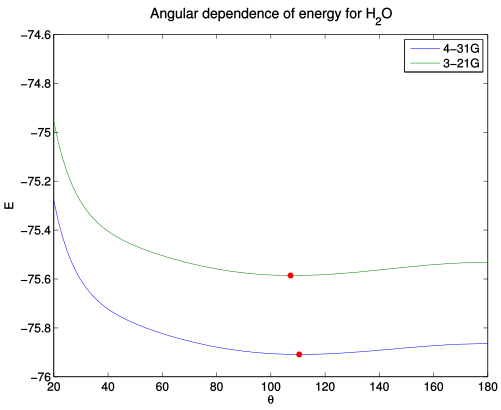
\includegraphics[width=0.5\textwidth]{figures/H2O_angular_energy.pdf}
\caption{Energy of H$_2$O plotted against the bond angle for two different basis sets, using $r=1.809$.}
\label{fig:eangularh2o}
\end{figure}

\begin{figure}
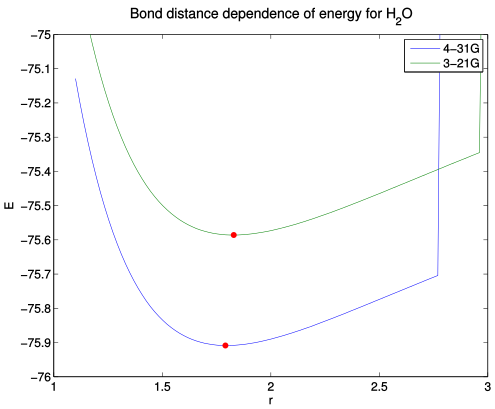
\includegraphics[width=0.5\textwidth]{figures/H2O_distance_energy.pdf}
\caption{Energy of H$_2$O plotted against the bond distance, using $\theta=111^\circ$ for 4-31G and 107 for 3-21G. The divergent behavior for long distances is because the Hartree-Fock solver did not converge.}
\label{fig:distanceh2o}
\end{figure}

An immidiate reaction to these results, is that the energy difference due to a change of basis, is an order of magnitude larger than the energy differences due to substantial changes in the nuclei configuration. We also see that the radial potential is stronger than the angular. This probably explains why H-O-H bending absorbs electromagnetic radiation at a higher freqency than O-H stretching \cite{Wikipedia}.

Just for a proof-of-concept, I include a grid-plot of energy as a function of both bond angle and bond distance, which is figure \ref{fig:configh2o}. The plot is surprisingly smooth, so I think a proper minimization scheme would converge quite easily to a very precise configuration $(r, \theta)$.

\begin{figure}
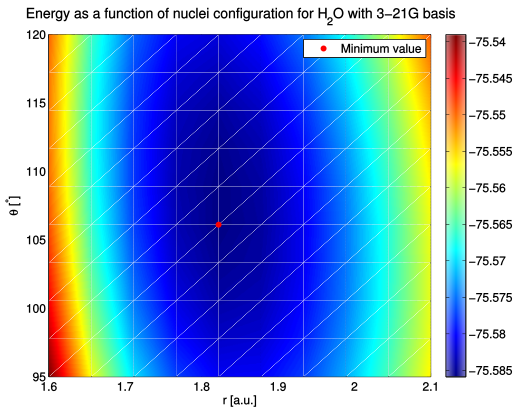
\includegraphics[width=0.5\textwidth]{figures/H2Oconfig_321g.pdf}
\caption{Energy as a function of nuclei configuration for H$_2$O with a 3-21G basis. The plot is slightly interpolated, and is derived from a 10x10 point grid in $r$ and $\theta$.}
\label{fig:configh2o}
\end{figure}


\section{Electron densities}
Figures \ref{fig:density1}, \ref{fig:density2}, \ref{fig:density3}, \ref{fig:density4}, \ref{fig:density5} and \ref{fig:density6} show electron densities for selected systems. We see that the distribution of electron density varies substantially among the systems. For atoms, it is very localised near the nucleus. H$_2$ for instance, has a density that is rather distributed among the nuclei \emph{and} in between the nuclei. We can conclude that the covalent bond in the hydrogen bond is strong. For the beryllium molecule, there are two very distinct peaks at the two nuclei, which indicates weaker bond than for the hydrogen atom. For water and silicon dioxide, we see another qualitatively different picture, where almost all electron desity is localized near one of the nuclei, O and Si respectively. 



\begin{figure}[h!tb]
\includegraphics[width=0.5\textwidth]{./figures/H2density_sto3g.pdf}
\caption{Electron density for H$_2$ with STO3G basis functions on all atoms}
\label{fig:density1}
\end{figure}

\begin{figure}[h!tb]
\includegraphics[width=0.5\textwidth]{./figures/Be2density_sto3g.pdf}
\caption{Electron density for Be$_2$ with STO-3G basis functions on all atoms}
\label{fig:density2}
\end{figure}

\begin{figure}[h!tb]
\includegraphics[width=0.5\textwidth]{./figures/Ardensity_321g.pdf}
\caption{Electron density for Ar with 3-21G basis functions on all atoms}
\label{fig:density3}
\end{figure}

\begin{figure}[h!tb]
\includegraphics[width=0.5\textwidth]{./figures/Nedensity_321g.pdf}
\caption{Electron density for Ne with 3-21G basis functions on all atoms}
\label{fig:density4}
\end{figure}

\begin{figure}[h!tb]
\includegraphics[width=0.5\textwidth]{./figures/H2Odensity_431g.pdf}
\caption{Electron density for H$_2$O with 4-31G basis functions on all atoms}
\label{fig:density5}
\end{figure}

\begin{figure}[h!tb]
\includegraphics[width=0.5\textwidth]{./figures/H2Odensity_321g.pdf}
\caption{Electron density for H$_2$O with 3-21G basis functions on all atoms}
\label{fig:density6}
\end{figure}

\begin{figure}[h!tb]
\includegraphics[width=0.5\textwidth]{./figures/SiO2density_321g.pdf}
\caption{Electron density for SiO$_2$ with 3-21G basis functions on all atoms. This is just an illustration of Hartree-Fock used on silicon dioxide. The configuration used is $\theta=144$ and $r = 3.062$ a.u. The energy caculated in this simulation in -3.08609 Hartree}
\end{figure}

\section{Discussion and interpretations}

\subsection{SiO$_2$}
It turns out that performing Hartree-Fock calculations on the SiO$_2$ molecule is not trivial. Silicon dioxide is mainly found in various crystal structures, where the equilibrium configuration is determined by the details of that crystal structure. The equilibrium configuration of one particular aton will thus be deremined by the presence of other atoms i a crystal. Also, I was not able to make the program fast enough to make an energy plot like the one for H$_2$O, but this is possible to do in principle. 

\subsection{Bond enthalpies for homonuclear molecules}
In the section on electron densities, I suggested that the bond energy is higher for the hydrogen molecule than for the beryllium molecule by looking qualitatively at the density plots. Chemists call this energy the bond enthalpy, and according to \cite{lide2004crc}, the bond enthalpy for Be-Be in Be$_2$ is 59 kJ/mol, while for H-H in H$_2$ it is 435.990 kJ/mol. It is of course not certain that it is the shape of the density distribution that causes this, but it seems reasonable. For Be$_2$, this is probably only interesting for theoretical purposes, as Beryllium does not like to form Be$_2$.

\subsection{Use of contracted basis sets}
Almost all the cpu-time is spent calculating integrals over primitives. This calculation is of order seconds or minutes on a desktop computer for systems of 2-3 particles. The self-consistent linear algebra problem to be solved after the integrals is done in much less than a second. Therefore, it is valid to question whether one shold use contracted orbitals, and not just optimize coefficients for all the primitives. The cpu-time would be the same, since all primitives has to be combined for all integrals. A possible reason for using contracted orbitals, is that it makes it easier for the HF-method to converge. We see already for the 4-31G and 3-21G basis set for water, that convergence problems occur. The alternative to doing a 4-31G would be 20 (4 s-orbitals + (3+1) s-orbitals + (3+1)*3 p-orbitals) individual orbitals, instead of 9 contracted, which would make convergence even harder. 


\subsection{Perspectives for future work}
It would be interesting to be able to look at bigger systems. In particular, it would be interesting to look at the behavior of the particle density of one molecule in the presence of another molecule or atom. This can for example give a better understanding of how silicon dioxide in crystal form behaves in the presence of water and vice versa, and also to calculate properties of different crystal forms of silicon dioxide. This requires the ability to look at larger systems, preferably periodic, and thus require parallellization of the code, and substantial rewriting to improve efficiency. 

\bibliography{mendeleybib}



\begin{appendix}

\section{The Slater determinant}
From here on follows what did not fit into the main text. It is here essentially to answer problem 1a in the project text.

Since electrons are indistinguishable, the Hamiltonian commutes with the particle-exchange operator $P_{ij}$:
\begin{equation}
	\Pvec_{ij}\Psi(\xvec_1, \xvec_2, ..., \xvec_i, ..., \xvec_j, ... \xvec_N) = \Psi(\xvec_1, \xvec_2, ..., \xvec_j, ..., \xvec_i, ... \xvec_N)
\end{equation}

The eigenvalue of $P$ is $-1$ (experimental) for fermions. We are working with an independent-particle Hamiltonian, so the electron state can be written as a product of single-electron states:
\begin{equation}
	\Psi(\xvec_1, ..., \xvec_N) = \psi_1(\xvec_1)\cdots\psi_N(\xvec_N)
\end{equation}

Many-electron states are required to be antisymmetrical with respect to the particle exchange. We assume the many-body elevtronic state to take form of an anti-symmetrized sum of permutations of the single-particle wave function. 

\begin{equation}
	\Psi_{AS} (\xvec_1, ..., \xvec_N) = \frac{1}{\sqrt{N!}} \sum_\mb{P} \epsilon_P \mb{P} \psi_1(\xvec_1) \cdots \psi_N(\xvec_N)
\end{equation}

This is known as a slater determinant.

\section{Bases and transformations}
We start out by using spin-orbitals $\psi_k$ as a basis for our approximation to the many-body electronic wave function. We assume the basis functions are orthonormal, i.e. $\langle \psi_i, \psi_j \rangle = \delta_{ij}$. We can construct a new basis of spin-orbitals by applying a unitary transformation, given by a unitary matrix $\mb{C}$. Since unitary matrices preserve inner products, then the orthonormality property of tha basis is preserved through the unitary transformation. 


Let us then look at the relation between the slater determinant of $\{ \psi\}$ and that of $\{\psi'\}$:
We start by defining a matrix $\mb{M}$ as
\begin{equation}
	M_{ij} =\frac{1}{\sqrt{N!}} \psi_j(\xvec_i)
\end{equation}

We want to show that the Slater determinant constructed from the spin orbitals $\{\psi'\}$ can be written as the determinant of the matrix product $\mb{C}\mb{M}$. Remember $\det(AB) = \det(BA) = \det(BA^T)$, so we can work with $\mb{M}'=\mb{M}\mb{C^T}$.

If we write out this product, we find:
\begin{equation}
	(MC^T)_{ij} = \sum_{k} M_{ik} C_{jk}
\end{equation}
\begin{equation}
	= \sum_{k}\frac{1}{\sqrt{N!}}C_{jk}\psi_k(\xvec_i)
\end{equation}

We originally assumed $C$ to be taking $\{ \psi\}$ to $\{\psi'\}$, so:
\begin{equation}
	\psi_k' = \sum_{l=1}^N C_{kl} \psi_l
	\label{eq:basis_change}
\end{equation}
Which means
\begin{equation}
(MC^T)_{ij} = \frac{1}{\sqrt{N!}} \psi_j'(x_i)
\end{equation}
The determinant of this matrix will be the same as the Slater determinant constructed from the new basis $\{\psi'\}$.

Now we want to find the relation between $\det{M}$ and $\det{M'}$. They are different by a factor of $\det{C^T} = \det{C}$. Since $C$ is unitary, $|\det C| = 1$.
\end{appendix}



\end{document}
